\section{Základní rovnice teorie pružnosti}

V~této části budou představeny základní veličiny a rovnice nezbytné pro popis chování pružných těles. Zaměříme se na vektor posunutí, vektor napětí a vektor deformací. Dále popíšeme geometrické, fyzikální a statické rovnice, které jsou klíčové pro pochopení základních principů pružnosti. Na závěr uvedeme okrajové podmínky.

\subsection{Přehled základních veličin}

\subsubsection*{Vektor posunutí}
Posunutí libovolného bodu pružného tělesa v~prostoru můžeme rozložit do tří vzájemně kolmých složek, které je možné zapsat ve formě vektoru posunutí~\cite[2]{teorie_pruznosti}

\begin{equation}
    \gls{u} 
    = 
    \begin{Bmatrix}
        \gls{u_i}[ ] & \gls{v_i}[ ] & \gls{w_i}[ ]
    \end{Bmatrix}^\mathrm{T}.
\end{equation}

\subsubsection*{Vektor deformací}
Každé z~uvedených napětí pracuje na odpovídající poměrné deformaci, normálovému napětí \gls{sigma_i}[i] odpovídá poměrná deformace \gls{eps_i}[i] a smykovému
napětí \gls{tau_i}[ij] odpovídá zkosení \gls{gamma_i}[ij]. Poměrné deformace je možné zapsat v~podobě vektoru poměrných deformací \cite[3]{teorie_pruznosti}

\begin{equation}
    \gls{eps}
    =
    \begin{Bmatrix}
        \gls{eps_i}[\gls{x}] &
        \gls{eps_i}[\gls{y}] &
        \gls{eps_i}[\gls{z}] &
        \gls{gamma_i}[\gls{y}\gls{z}] &
        \gls{gamma_i}[\gls{z}\gls{x}] &
        \gls{gamma_i}[\gls{x}\gls{y}]
    \end{Bmatrix}^\mathrm{T}.
\end{equation}

\subsubsection*{Vektor napětí}
Na obrázku \ref{fig:point_stress} jsou zobrazena napětí v~materiálovém bodě tělesa. Ve směru jednotlivých os systému souřadnic působí tři normálová napětí \gls{sigma_i}[\gls{x}], \gls{sigma_i}[\gls{y}] a \gls{sigma_i}[\gls{z}]. Rovnoběžně s~osami systému působí šest smykových napětí v~rovinách \gls{x}\gls{y}, \gls{y}\gls{z}, \gls{z}\gls{x} \cite[2]{teorie_pruznosti}.

\begin{figure}[H]
    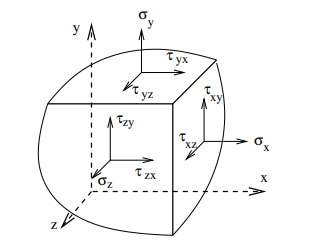
\includegraphics[height=5cm]{assets/figures/framesss/point_stress.png}
    \caption[Napětí v~materiálovém bodě]{Napětí v~materiálovém bodě, převzato z~\cite[3]{teorie_pruznosti}}
    \label{fig:point_stress}
\end{figure}

Uplatněním předpokladu o~vzájemnosti smykových napětí, je možné považovat jen tři smyková napětí za nezávislá \cite[3]{teorie_pruznosti}.

\begin{equation}
    \begin{aligned}
        \gls{tau_i}[\gls{x}\gls{y}] = \gls{tau_i}[\gls{y}\gls{x}], \\
        \gls{tau_i}[\gls{y}\gls{z}] = \gls{tau_i}[\gls{z}\gls{y}], \\
        \gls{tau_i}[\gls{x}\gls{z}] = \gls{tau_i}[\gls{z}\gls{x}].
    \end{aligned}
\end{equation}

Složky lze zapsat v~podobě vektoru napětí

\begin{equation}
    \gls{sigma} 
    =
    \begin{Bmatrix}
        \gls{sigma_i}[\gls{x}] &
        \gls{sigma_i}[\gls{y}] &
        \gls{sigma_i}[\gls{z}] &
        \gls{tau_i}[\gls{y}\gls{z}] &
        \gls{tau_i}[\gls{z}\gls{x}] &
        \gls{tau_i}[\gls{x}\gls{y}]
    \end{Bmatrix}^\mathrm{T}.
\end{equation}

\subsection{Přehled základních rovnic}

\subsubsection*{Geometrické rovnice}
Tělesa mění z~nejrůznějších příčin svůj tvar a objem -- deformují se. Pro deformaci elementárního kvádru jsou typické dva základní geometricko-deformační modely. První předpokládá protažení hran kvádru ve směrech souřadnicových os při zachování pravých úhlů mezi stěnami a druhý model se vyznačuje změnami pravých úhlů mezi stěnami kvádru při zachování délek hran \cite[9]{prpe10}. Na obr. \ref{fig:elementary_block} je pro názornost nakreslen pouze průmět kvádru do roviny \gls{x}\gls{y}.

\begin{figure}[H]
    \begin{tikzpicture}[>={Stealth[inset=0pt,length=8pt,angle'=28,round]}]

    \draw[->] (-0.5, -0.5) -- (8.5, -0.5) node[above] {$\gls{x}, \gls{u_i}[ ]$};
    \draw[->] (-0.5, -0.5) -- (-0.5, 7) node[left] {$\gls{y}, \gls{v_i}[ ]$};

    \coordinate (A_u) at (2.5, 2.5);
    \coordinate (B_u) at (6.5, 2.5);
    \coordinate (C_u) at (6.5, 5);
    \coordinate (D_u) at (2.5, 5);

    
    \coordinate (A_bar) at (2.5, 2.5);
    \coordinate (B_bar) at (7.5, 3.5); 
    \coordinate (C_bar) at (8.5, 7);
    \coordinate (D_bar) at (3.5, 6);

    \draw[draw=ctublue, line width=0.5mm, fill=ctulightblue!30] (A_bar) -- (B_bar) -- (C_bar) -- (D_bar) -- cycle;
    \draw[dotted, draw=ctublue, line width=0.25mm] (A_u) rectangle (C_u);

    \node[above right, color=ctublue] (A_bar_txt) at (A_bar) {$\mathrm{A'}$};
    \node[above left, color=ctublue] (B_bar_txt) at (B_bar) {$\mathrm{B'}$};
    \node[below left, color=ctublue] (C_bar_txt) at (C_bar) {$\mathrm{C'}$};
    \node[below right, color=ctublue] (D_bar_txt) at (D_bar) {$\mathrm{D'}$};
    
    \coordinate (A) at (1, 1);
    \coordinate (B) at (5, 1);
    \coordinate (C) at (5, 3.5);
    \coordinate (D) at (1, 3.5);

    \node at (A) [below left] {A};
    \node at (B) [below right] {B};
    \node at (C) [above right] {C};
    \node at (D) [above left] {D};

    \draw[draw=black, line width=0.5mm] (A) rectangle (C);
    
    \draw[|<->|, draw=black] (1, 0.25) -- node[above] {$\dd{\gls{x}}$} ++ (4, 0);
    \draw[|<->|, draw=black] (0.25, 1) -- node[left] {$\dd{\gls{y}}$} ++(0, 2.5);


    \draw[|<->|, draw=black] (1,1.75) -- node[above left] {\gls{u_i}[ ]} ++(1.5, 0);
    \draw[<->|, draw=black] (2.5, 1.75) -- node[above] {$\dd{\gls{x}}$} ++ (4, 0);
    \draw[<->|, draw=black] (6.5, 1.75) -- node[above] {$\pdv{\gls{u_i}[ ]}{\gls{x}}\dd{\gls{x}}$} ++(1, 0);

    \draw[<->|, draw=black] (2, 1) -- node[below left] {\gls{v_i}[ ]} ++(0, 1.5);
    \draw[<->|, draw=black] (2, 2.5) -- node[left] {$\dd{\gls{y}}$} ++(0, 2.5);
    \draw[<->|, draw=black] (2, 5) -- node[left] {$\pdv{\gls{v_i}[ ]}{\gls{y}}\dd{\gls{y}}$} ++(0, 1);

    \draw[|<->|, draw=black] (8, 2.5) -- node[right] {$\pdv{\gls{v_i}[ ]}{\gls{x}}\dd{\gls{x}}$} ++(0, 1);

    \draw[|<->|, draw=black] (8, 2.5) -- node[right] {$\pdv{\gls{v_i}[ ]}{\gls{x}}\dd{\gls{x}}$} ++(0, 1);
    \draw[|<->|, draw=black] (2.5, 6.5) -- node[above] {$\pdv{\gls{u_i}[ ]}{\gls{y}}\dd{\gls{y}}$} ++(1, 0);

    \draw[|<->|,domain=0:11.31, draw=black] plot ({2.5+3.5*cos(\x)}, {2.5+3.5*sin(\x)});
    \node at (5.7, 2.8) {$\alpha$};

    \draw[|<->|, domain=90:90-15.95, draw=black] plot ({2.5+2.2*cos(\x)}, {2.5+2.2*sin(\x)});
    \node at (2.75, 4.3) {$\beta$};

\end{tikzpicture}
    \caption[Deformace elementárního kvádru]{Deformace elementárního kvádru, podle \cite[obr. 1.2]{teorie_pruznosti}}
    \label{fig:elementary_block}
\end{figure}

Prodloužení kvádru ve směru \gls{x} můžeme vyjářit následovně

\begin{equation}
    \gls{eps_i}[x] 
    = 
    \frac{|\mathrm{A'B'}| - |\mathrm{AB}|}{|\mathrm{AB}|}
    =
    \frac{\left(\dd{\gls{x}} + \pdv{\gls{u_i}[ ]}{\gls{x}} \dd{\gls{x}}\right) - \dd{\gls{x} }}{\dd{\gls{x}}}
    =
    \pdv{\gls{u_i}[ ]}{\gls{x}}.
\end{equation}

Analogicky lze získat vztahy pro \gls{eps_i}[\gls{y}] a \gls{eps_i}[\gls{z}]. Shrnutí vztahů pro poměrné prodloužení ve směru souřadnicových os je uvedeno v~\ref{eq:normal_strain}.

\begin{equation}
    \label{eq:normal_strain}
    \begin{aligned}
        \gls{eps_i}[\gls{x}] & = \pdv{\gls{u_i}[ ]}{\gls{x}}, \\
        \gls{eps_i}[\gls{y}] & = \pdv{\gls{v_i}[ ]}{\gls{y}}, \\
        \gls{eps_i}[\gls{z}] & = \pdv{\gls{w_i}[ ]}{\gls{z}}.
    \end{aligned}
\end{equation}

Smykové zkosení je možné stanovit na základě určení velikostí úhlů $\alpha$ a $\beta$ na obr. \ref{fig:elementary_block}, zavedeme předpoklad, že $\tan{\alpha} = \alpha$, $\tan{\beta}=\beta$, $\pdv{\gls{u_i}[ ]}{\gls{x}} \dd{\gls{x}} = 0$ a $\pdv{\gls{v_i}[ ]}{\gls{y}}\dd{\gls{y}} = 0$.

\begin{equation}
    \gls{gamma_i}[\gls{x}\gls{y}]
    =
    \alpha + \beta
    \approx
    \frac{\pdv{\gls{v_i}[ ]}{\gls{x}}\dd{\gls{x}}}{\dd{\gls{x}}}
    +
    \frac{\pdv{\gls{u_i}[ ]}{\gls{y}}\dd{\gls{y}}}{\dd{\gls{y}}}
    =
    \pdv{\gls{v_i}[ ]}{\gls{x}} + \pdv{\gls{u_i}[ ]}{\gls{y}}
    .
\end{equation}

Analogicky lze zapsat vztahy pro zbývající smyková zkosení

\begin{equation}
    \begin{aligned}
        \gls{gamma_i}[\gls{x}\gls{y}] & = \gls{gamma_i}[\gls{y}\gls{x}] = \pdv{\gls{v_i}[ ]}{\gls{x}} + \pdv{\gls{u_i}[ ]}{\gls{y}}, \\
        \gls{gamma_i}[\gls{y}\gls{z}] & = \gls{gamma_i}[\gls{z}\gls{y}] = \pdv{\gls{w_i}[ ]}{\gls{y}} + \pdv{\gls{v_i}[ ]}{\gls{z}}, \\
        \gls{gamma_i}[\gls{z}\gls{x}] & = \gls{gamma_i}[\gls{x}\gls{z}] = \pdv{\gls{u_i}[ ]}{\gls{z}} + \pdv{\gls{w_i}[ ]}{\gls{x}}.
    \end{aligned}
\end{equation}

\subsubsection*{Fyzikální rovnice}

Jako fyzikální vztahy se označují vztahy mezi napětím a poměrnými deformacemi. Jak je známo z~pružnosti, poměr mezi podélnou a příčnou změnou délky tělesa je konstantní a je popsán Poissonovým součinitelem \gls{nu}. Potom je na místě předpokládat, že velikost poměrného prodloužení \gls{eps_i}[\gls{x}] bude ovlivněna nejen napětím \gls{sigma_i}[\gls{x}], ale v~závislosti na hodnotě \gls{nu} také napětím ve směrech \gls{y} a \gls{z} \cite[7]{teorie_pruznosti}

\begin{equation}
    \gls{eps_i}[\gls{x}] = \frac{1}{\gls{E}} \left[ \gls{sigma_i}[\gls{x}] - \gls{nu} (\gls{sigma_i}[\gls{y}] + \gls{sigma_i}[\gls{z}])  \right].
\end{equation}

U~smyku lze předpokládat, že vztah mezi smykovým napětím \gls{tau_i}[ij] a zkosením \gls{gamma_i}[ij] bude lineární

\begin{equation}
    \gls{gamma_i}[ij] = \frac{\gls{tau_i}[ij]}{2 \gls{G}}.
\end{equation}

Fyzikální vztahy pro pružné těleso v~prostoru můžeme zapsat ve tvaru

\begin{equation}
    \begin{aligned}
        \gls{eps_i}[\gls{x}] & = \frac{1}{\gls{E}} \left[ \gls{sigma_i}[\gls{x}] - \gls{nu} (\gls{sigma_i}[\gls{y}] + \gls{sigma_i}[\gls{z}])  \right], 
        & \quad \gls{gamma_i}[\gls{y}\gls{z}] & = \frac{\gls{tau_i}[\gls{y}\gls{z}]}{2 \gls{G}}, \\
        \gls{eps_i}[\gls{y}] & = \frac{1}{\gls{E}} \left[ \gls{sigma_i}[\gls{y}] - \gls{nu} (\gls{sigma_i}[\gls{x}] + \gls{sigma_i}[\gls{z}])  \right],
        & \quad \gls{gamma_i}[\gls{x}\gls{z}] & = \frac{\gls{tau_i}[\gls{x}\gls{z}]}{2 \gls{G}}, \\
        \gls{eps_i}[\gls{z}] & = \frac{1}{\gls{E}} \left[ \gls{sigma_i}[\gls{z}] - \gls{nu} (\gls{sigma_i}[\gls{y}] + \gls{sigma_i}[\gls{x}])  \right], 
        & \quad \gls{gamma_i}[\gls{x}\gls{y}] & = \frac{\gls{tau_i}[\gls{x}\gls{y}]}{2 \gls{G}}.
    \end{aligned}
\end{equation}

\subsubsection*{Statické rovnice}
V~případě pružného tělesa je vhodné napsat silové podmínky rovnováhy na vyjmutém diferenciálním objemu o~rozměrech $\dd{\gls{x}}$, $\dd{\gls{y}}$, $\dd{\gls{z}}$, který je zobrazen na obrázku \ref{fig:stresses} \cite[6]{teorie_pruznosti}.

Pro lepší přehlednost jsou napětí označená jako $\gls{sigma_i}[i]'$ a $\gls{tau_i}[ij]'$ napětí změněná o~přírůstek na diferenciálním rozměru objemu, tedy například

\begin{equation}
    \label{eq:equilibrium_eq_helpers}
    \gls{sigma_i}[\gls{x}]' = \gls{sigma_i}[\gls{x}] + \pdv{\gls{sigma_i}[\gls{x}]}{\gls{x}} \dd{\gls{x}},
    \quad
    \gls{tau_i}[\gls{x}\gls{y}]' = \gls{tau_i}[\gls{x}\gls{y}] + \pdv{\gls{tau_i}[\gls{x}\gls{y}]}{\gls{y}} \dd{\gls{y}}, \, \dots
\end{equation}

\begin{figure}[H]
    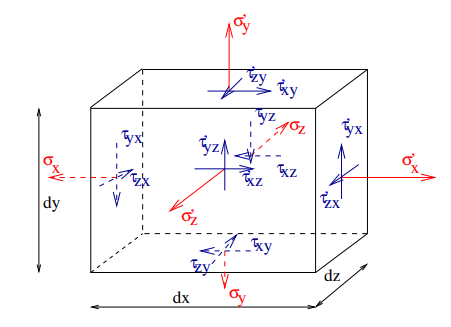
\includegraphics[height=6cm]{assets/figures/framesss/stresses.png}
    \caption[Napětí na diferenciálním výseku tělesa]{Napětí na diferenciálním výseku tělesa, převzato z~\cite[5]{teorie_pruznosti}}
    \label{fig:stresses}
\end{figure}

Výslednice napětí \gls{sigma_i}[\gls{x}] se získá vynásobením napětí a plochy na které působí,

\begin{equation}
    F_{\gls{sigma_i}[ ],\gls{x}} = \gls{sigma_i}[\gls{x}] \dd{\gls{y}} \dd{\gls{z}}.
\end{equation}

Silovou podmínku rovnováhy ve směru osy \gls{x} je možné zapsat jako

\begin{equation}
    \label{eq:equilibrium_eq}
    \sum{F_{i,\gls{x}}} = (\gls{sigma_i}[\gls{x}]' - \gls{sigma_i}[\gls{x}]) \dd{\gls{y}} \dd{\gls{z}}
    + (\gls{tau_i}[\gls{x}\gls{y}]' - \gls{tau_i}[\gls{x}\gls{y}]) \dd{\gls{x}} \dd{\gls{z}}
    + (\gls{tau_i}[\gls{x}\gls{z}]' - \gls{tau_i}[\gls{x}\gls{z}]) \dd{\gls{x}} \dd{\gls{y}} = 0.
\end{equation}

Rozepsáním rovnice \ref{eq:equilibrium_eq} pomocí vztahů \ref{eq:equilibrium_eq_helpers} dostaneme výraz

\begin{equation}
    \begin{aligned}
        & \left(
            \gls{sigma_i}[\gls{x}] 
            - \gls{sigma_i}[\gls{x}] 
            - \pdv{\gls{sigma_i}[\gls{x}]}{\gls{x}} \dd{\gls{x}}
        \right) \dd{\gls{y}} \dd{\gls{z}} \\
        & +
        \left(
            \gls{tau_i}[\gls{x}\gls{y}]
            - \gls{tau_i}[\gls{x}\gls{y}]
            - \pdv{\gls{tau_i}[\gls{x}\gls{y}]}{\gls{y}} \dd{\gls{y}}
        \right) \dd{\gls{x}} \dd{\gls{z}} \\
        & +
        \left(
            \gls{tau_i}[\gls{x}\gls{z}]
            - \gls{tau_i}[\gls{x}\gls{z}]
            - \pdv{\gls{tau_i}[\gls{x}\gls{z}]}{\gls{z}} \dd{\gls{z}}
        \right) \dd{\gls{x}} \dd{\gls{y}}
        = 0,
    \end{aligned}
\end{equation}

který lze dále upravit na

\begin{equation}
    \pdv{\gls{sigma_i}[\gls{x}]}{\gls{x}}
    +
    \pdv{\gls{tau_i}[\gls{x}\gls{y}]}{\gls{y}}
    +
    \pdv{\gls{tau_i}[\gls{x}\gls{z}]}{\gls{z}}
    = 0.
\end{equation}

Obdobně lze napsat podmínky rovnováhy o~pro směry \gls{y} a \gls{z}. Takto sestavené rovnice doplníme o~objemové síly $X$, $Y$ a $Z$, působící ve směrech jednotlivých souřadnicových os, získáme výsledný tvar podmínek rovnováhy,

\begin{equation}
    \begin{aligned}
        \pdv{\gls{sigma_i}[\gls{x}]}{\gls{x}}
        +
        \pdv{\gls{tau_i}[\gls{x}\gls{y}]}{\gls{y}}
        +
        \pdv{\gls{tau_i}[\gls{x}\gls{z}]}{\gls{z}}
        + X & = 0, \\
        \pdv{\gls{tau_i}[\gls{x}\gls{y}]}{\gls{x}}
        +
        \pdv{\gls{sigma_i}[\gls{y}]}{\gls{y}}
        +
        \pdv{\gls{tau_i}[\gls{y}\gls{z}]}{\gls{z}}
        + Y & = 0, \\
        \pdv{\gls{tau_i}[\gls{z}\gls{x}]}{\gls{x}}
        +
        \pdv{\gls{tau_i}[\gls{z}\gls{y}]}{\gls{y}}
        +
        \pdv{\gls{sigma_i}[\gls{z}]}{\gls{z}}
        + Z~& = 0.
    \end{aligned}
\end{equation}

\subsection{Okrajové podmínky}

Složky napětí \gls{sigma} i složky posunutí \gls{eps} musí vyhovovat okrajovým podmínkám předepsaným na hranici tělesa $\gls{gamma} = \gls{gamma_p} + \gls{gamma_u}$.

\subsubsection*{Statické okrajové podmínky}
Statické okrajové podmínky tvoří soustavu tří lineárních algebraických rovnic a vyžadují požadavek rovnováhy pole napětí \gls{sigma} s~předepsaným zatížením \gls{p_bar} na části hranice \gls{gamma_p} \cite[35]{prpe10}. V~maticovém tvaru je lze zapsat

\begin{equation}
    \begin{bmatrix}
        n_{\gls{x}} & 0 & 0 & 0 & n_{\gls{z}} & n_{\gls{y}} \\
        0 & n_{\gls{y}} & 0 & n_{\gls{z}} & 0 & n_{\gls{x}} \\
        0 & 0 & n_{\gls{z}} & n_{\gls{y}} & n_{\gls{z}} & 0
    \end{bmatrix}
    \begin{Bmatrix}
        \gls{sigma_i}[\gls{x}] \\
        \gls{sigma_i}[\gls{y}] \\
        \gls{sigma_i}[\gls{z}] \\
        \gls{tau_i}[\gls{y}\gls{z}] \\
        \gls{tau_i}[\gls{z}\gls{x}] \\
        \gls{tau_i}[\gls{x}\gls{y}]
    \end{Bmatrix}
    =
    \begin{Bmatrix}
        \overline{p}_{\gls{x}} \\
        \overline{p}_{\gls{y}} \\
        \overline{p}_{\gls{z}} \\ 
    \end{Bmatrix},
\end{equation}

neboli

\begin{equation}
    \label{eq:static_boundary_conditions}
    \gls{normal_matrix} \gls{sigma} = \gls{p_bar} \quad \text{na \gls{gamma_p}}.
\end{equation}


\subsubsection*{Kinematické okrajové podmínky}
Kinematické (geometrické) okrajové podmínky se vztahují na část hranice \gls{gamma_u}, kde jsou předepsány posuny $\gls{u_bar} = \begin{Bmatrix}
    \overline{\gls{u_i}[ ]} & \overline{\gls{v_i}[ ]} & \overline{\gls{w_i}[ ]}
\end{Bmatrix}^{\mathrm{T}}$ a mají tvar

\begin{equation}
    \gls{u} = \gls{u_bar} \quad \text{na \gls{gamma_u}}.
\end{equation}

\subsection{Shrnutí}

Pro úplný popis chování pružného tělesa je v~každém jeho bodě potřeba získat hodnoty 15 neznámých veličin, 3 složky posunutí \gls{u}, 6 složek deformací \gls{eps} a 6 složek napětí \gls{sigma}. K~jejich vypočtení máme k~dispozici 15 rovnic, 6 geometrických rovnic, 6 fyzikálních rovnic a 3 statické rovnice (podmínky rovnováhy) \cite[8]{teorie_pruznosti}.

Zmíněné rovnice lze zapsat v~kompaktním tvaru:
\begin{alignat}{2}
    \text{statické~rovnice} \quad && \boldsymbol\partial \gls{sigma}^\mathrm{T} + \gls{X_bar} &= \matr{0}, \label{eq:equilibrium_equations}\\
    \text{fyzikální~rovnice} \quad && \gls{sigma} &= \gls{D} \gls{eps}, \label{eq:constitutive_equations}\\
    \text{geometrické~rovnice} \quad && \gls{eps} &= \boldsymbol\partial{\gls{u}} \label{eq:kinematic_equations},
\end{alignat}
kde
\begin{alignat*}{2}
    & \text{\glsdesc{u}} 
    && \quad \gls{u}
        = 
        \begin{Bmatrix}
            \gls{u_i}[ ] & \gls{v_i}[ ] & \gls{w_i}[ ]
        \end{Bmatrix}^\mathrm{T},
    \\
    & \text{\glsdesc{eps}} 
    && \quad \gls{eps}
        = \begin{Bmatrix}
            \gls{eps_i}[\gls{x}] &
            \gls{eps_i}[\gls{y}] &
            \gls{eps_i}[\gls{z}] &
            \gls{gamma_i}[\gls{x}\gls{y}] &
            \gls{gamma_i}[\gls{y}\gls{z}] &
            \gls{gamma_i}[\gls{z}\gls{x}]
        \end{Bmatrix}^\mathrm{T},
    \\
    %& \text{\glsdesc{D}}
    %&& \quad \gls{D} =
    %\\
    & \text{\glsdesc{sigma}}
    && \quad \gls{sigma}
        = \begin{Bmatrix}
            \gls{sigma_i}[\gls{x}] &
            \gls{sigma_i}[\gls{y}] &
            \gls{sigma_i}[\gls{z}] &
            \gls{tau_i}[\gls{x}\gls{y}] &
            \gls{tau_i}[\gls{y}\gls{z}] &
            \gls{tau_i}[\gls{z}\gls{x}]
        \end{Bmatrix}^\mathrm{T},
    \\
    & \text{\glsdesc{X_bar}}
    && \quad \gls{X_bar}
        = \begin{Bmatrix}
            $X$ & $Y$ & $Z$
        \end{Bmatrix}^\mathrm{T},
    \\ 
    & \text{operátorová matice}
    && \quad \boldsymbol{\partial}
        = \begin{bmatrix}
            \pdv{\gls{x}} & 0 & 0 & 0 & \pdv{\gls{z}} & \pdv{\gls{y}} \\
            0 & \pdv{\gls{y}} & 0 & \pdv{\gls{z}} & 0 & \pdv{\gls{x}} \\
            0 & 0 & \pdv{\gls{z}} & \pdv{\gls{y}} & \pdv{\gls{x}} & 0
        \end{bmatrix}^\mathrm{T},
    \\
    & \text{nulový vektor}
    && \quad \matr{0} = \begin{Bmatrix}
        0 & 0 & 0
    \end{Bmatrix}^\mathrm{T}.
\end{alignat*}

Postupný dosazením \ref{eq:kinematic_equations} a \ref{eq:constitutive_equations} do \ref{eq:equilibrium_equations} získáme silné řešení ve tvaru

\begin{equation}
    \label{eq:strong_form}
    \partial^{\mathrm{T}} \gls{D} \partial{\gls{u}} + \gls{X_bar} = \matr{0}.
\end{equation}

\begin{figure}[H]
    \begin{tikzpicture}[>={Stealth[inset=0pt,length=8pt,angle'=28,round]}]
        \tikzstyle{box} = [rectangle, minimum width=1cm, minimum height=1cm, text centered, draw=black, fill=ctulightblue!30]
    
        \node (displacement) [box] {\gls{u}};
        \node (strain) [box, below=3 cm of displacement] {\gls{eps}};
        \node (stress) [box, right=6 cm of strain] {\gls{sigma}};
        \node (forces) [box, above=3 cm of stress] {\gls{X_bar}};
    
        \draw[->] (displacement) -- node[fill=white] {$\gls{eps} = \partial{\gls{u}}$} (strain);
        \draw[->] (strain) -- node[fill=white] {$\gls{sigma} = \gls{D} \gls{eps}$} (stress);
        \draw[->] (stress) -- node[fill=white] {$\partial^{\mathrm{T}}\gls{sigma} + \gls{X_bar} = \matr{0}$} (forces);
        \draw[->] (forces) -- node[fill=white] (A) {$\partial^{\mathrm{T}} \gls{D} \partial{\gls{u}} + \gls{X_bar} = \matr{0}$} (displacement);
        \node[below=0.1cm of A] (B) {\gls{u} = \gls{u_bar} \quad \text{na \gls{gamma_u}}};
        \node[below=0.1cm of B] {\gls{normal_matrix} \gls{sigma} = \gls{p_bar} \quad \text{na \gls{gamma_p}}};
    
    \end{tikzpicture}
    \caption[Schéma vztahů základních rovnic teorie pružnosti a silného řešení]{Schéma vztahů základních rovnic teorie pružnosti a silného řešení, podle \cite[obr. 1.2]{fem_lourenco}}
    \label{fig:elasticity_diagram}
\end{figure}


\begin{citeQuote}{prpe10}[36]
    S~přesným řešením systému podmínečných rovnic se v~inženýrské praxi setkáváme poměrně zřídka. S~výjimkou několika speciálních typů konstrukcí, jako jsou prutové soustavy nebo rotačně symetrické a symetricky zatížené prostorové konstrukce (např. válcové, kulové ap.), je zpravidla třeba použít řešení přibližných.
\end{citeQuote}

\begin{citeQuote}{fem_lourenco}[kap. 1.1]
    According to solid mechanics, the solution must satisfy this set of differential equations with additional constraints (leading to the so called Boundary Value Problem). Closed-form solutions, such as ${\gls{u}(\gls{x_})=\begin{bmatrix}
        \gls{u_i}[ ](\gls{x_}) & \gls{v_i}[ ](\gls{x_}) & \gls{w_i}[ ](\gls{x_})
    \end{bmatrix}^{\mathrm{T}}}$ defined over the entire problem domain, are possible only when simple geometries and loadings are considered.
\end{citeQuote}